% SETUP
\documentclass[11pt]{article}
\linespread{1.1}
\usepackage[utf8]{inputenc}
\usepackage{graphicx, amsmath, array, graphics, amssymb, epsfig, psfrag, geometry, alltt, subfiles, blindtext, enumitem, pdfpages, float, mathtools}
\usepackage[export]{adjustbox}
\usepackage{fancyhdr}
\usepackage{array}
\usepackage{hyperref}
\geometry{a4paper, top = 20mm, bottom = 20mm, left = 15mm, right = 15mm}

% Headers
\pagestyle{fancy}
\fancyhf{}
\chead{ELEN90066 Embedded Systems Design - Assignment 2}
\cfoot{\thepage}

% Cover Sheet
\begin{document}

\includepdf{EngCSAss2.pdf}
\clearpage
\setcounter{page}{1}

% Title
\begin{center}
\textbf{\Large{Assignment 2}}\\
YiLin Inez Zheng [702279], \\
Workshop: Monday 3:15pm - 6:15pm, Due: 23/09/19  
\end{center}

\section*{Chapter 3 - page 73}
\subsection*{Exercise 2 (7 marks)}
\begin{enumerate}[label=\alph*)]
    \item %a
    Figure \ref{fig:Ch3Ex2} represents the temperature regulating FSM.
    \begin{figure}[H]
    \centering
    \textbf{Input}: $temperature$: numeric, $timer$: pure\\
    \textbf{Output}: $heating$: pure\\
    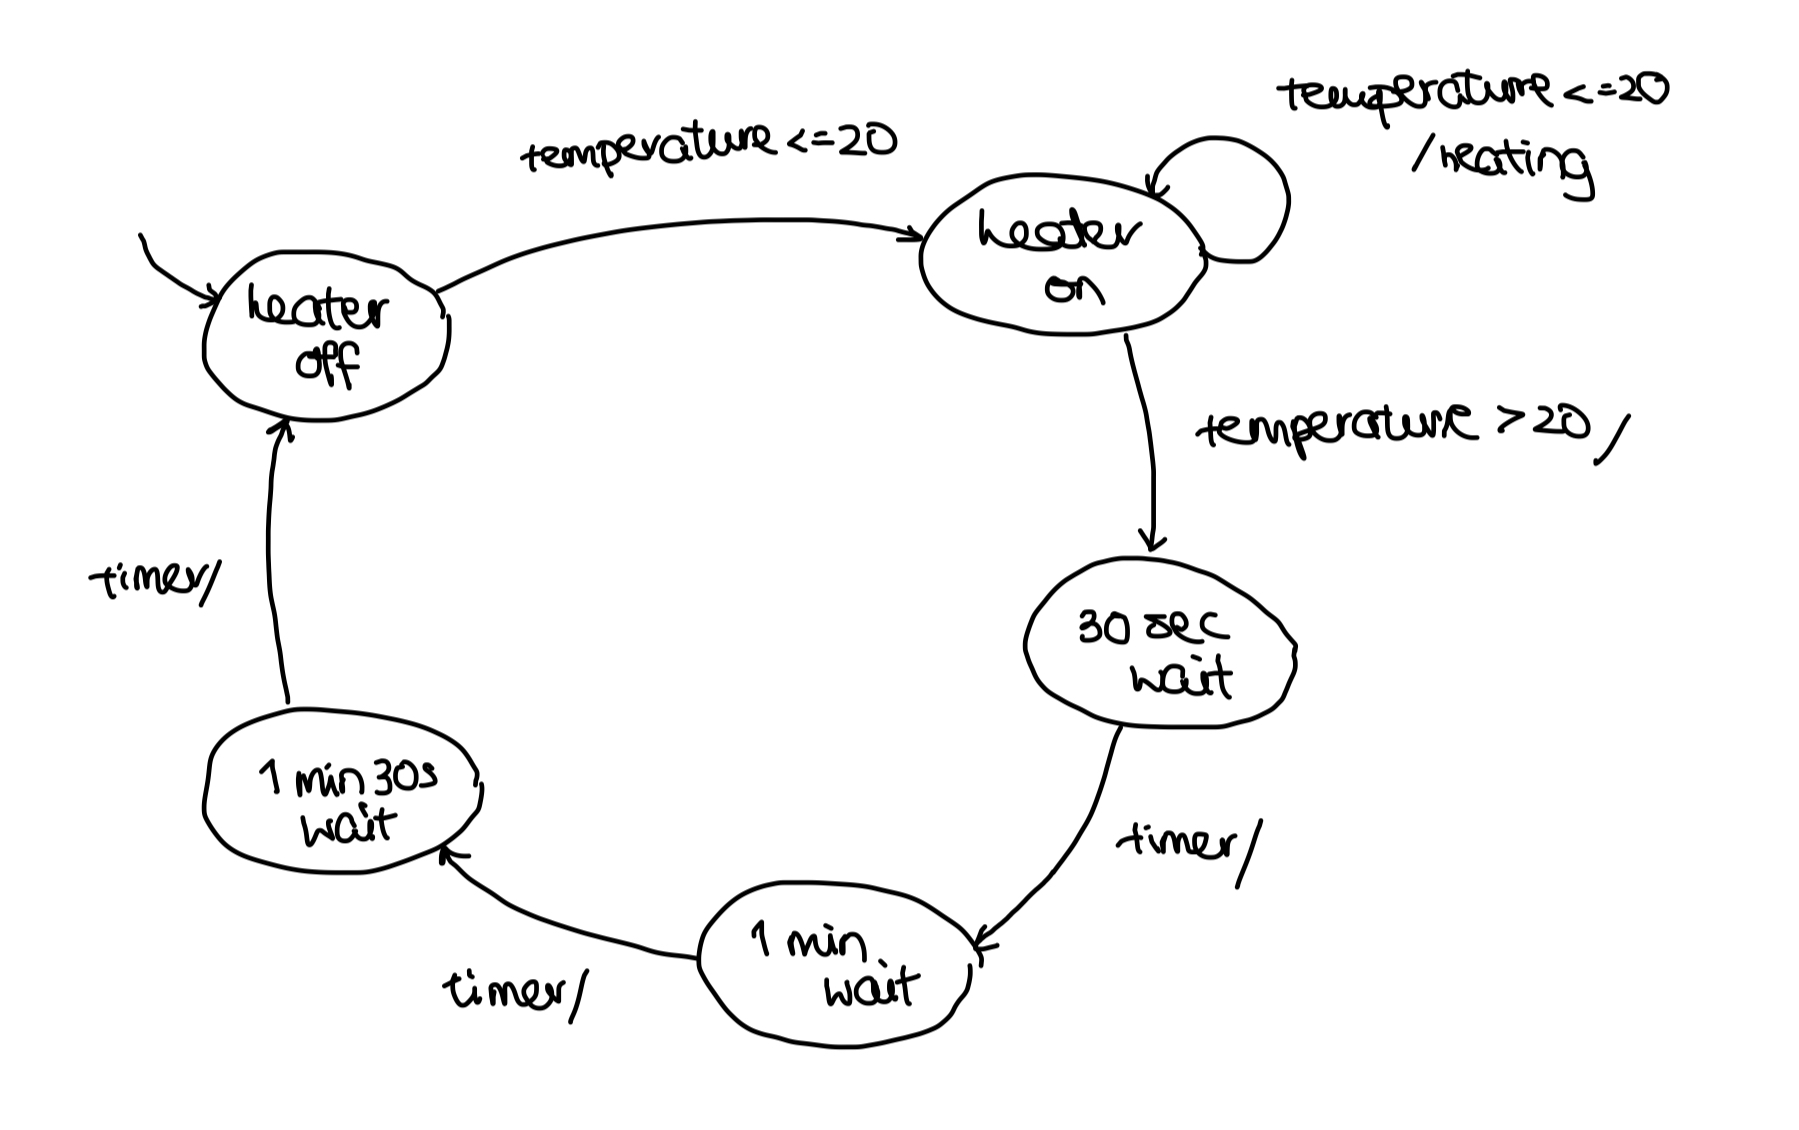
\includegraphics[width=10cm]{Ch3Ex2.jpeg}
    \caption{Temperature FSM}
    \label{fig:Ch3Ex2}
    \end{figure}
    \item %b
    5 states in my FSM. Should be the least because the system updates every 30 seconds, and therefore to track time, it requires 3 extra waiting states.  
    \item %c
    The machine is not time invariant. A fixed time is set for the heater on and off actions so if the input time is changed the output would be affected differently. 
\end{enumerate}
\subsection*{Exercise 4 (3 marks)}
All 3 states are reachable. The variable $n$ does not affect the transitions.
\subsection*{Exercise 5 (13 marks)}
\begin{enumerate}[label=\alph*)]
    \item %a 
    \begin{itemize}
        \item \textit{States}: \{red, green, yellow\}
        \item \textit{Inputs}: (\{\textit{tick}\} $\rightarrow$ \{\textit{present, absent}\})
        \item \textit{Outputs}: (\{\textit{go, stop}\} $\rightarrow$ \{\textit{present, absent}\})
        \item  
        $$update(s,tick) =  \begin{cases}
        (\text{green}, go) \hspace{3cm}\text{ if $s =$ red}\\
        (\text{yellow}, stop) \hspace{2.5cm}\text{ if $s =$ green}\\
        (\text{red}, stop) \hspace{3cm}\text{ if $s =$ yellow}
        \end{cases}$$
        \item \textit{initialState}: red
    \end{itemize}
    \item %b
    $(tick, \text{red}, go),(tick, \text{green}, stop), (tick, \text{yellow}, stop), (tick, \text{red}, go))$
    \item %c
    No it is not deterministic. The machine will reduce down to Figure \ref{fig:Ch3Ex5a} and the stop state will have a self transition leading to non-distinct output sequences. The trace of length 4 is shown in Figure \ref{fig:Ch3Ex5}. 
    \begin{figure}[H]
    \centering
    \textbf{Input}: green, stop: pure\\ 
    \textbf{Output}: $go$, $stop$: pure\\
    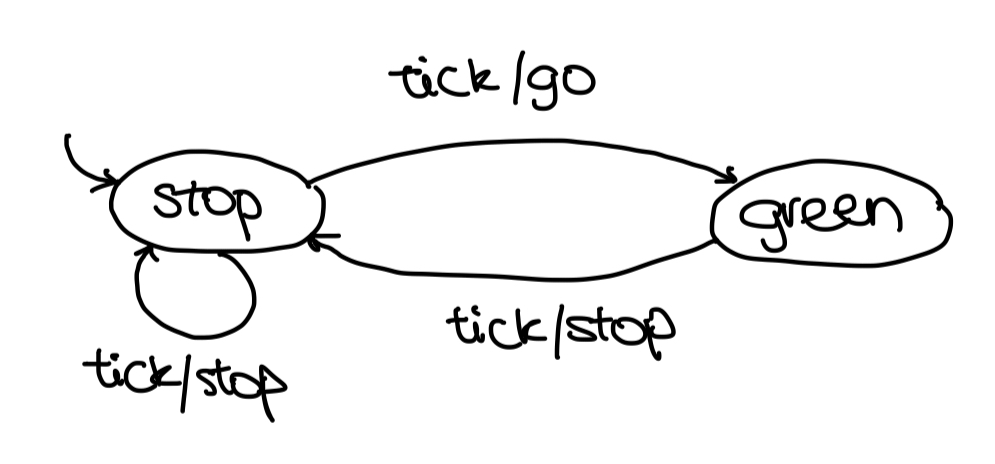
\includegraphics[width=6cm]{Ch3Ex5a.jpeg}
    \caption{Reduced state machine}
    \label{fig:Ch3Ex5a}
    \end{figure}
    \begin{figure}[H]
    \centering
    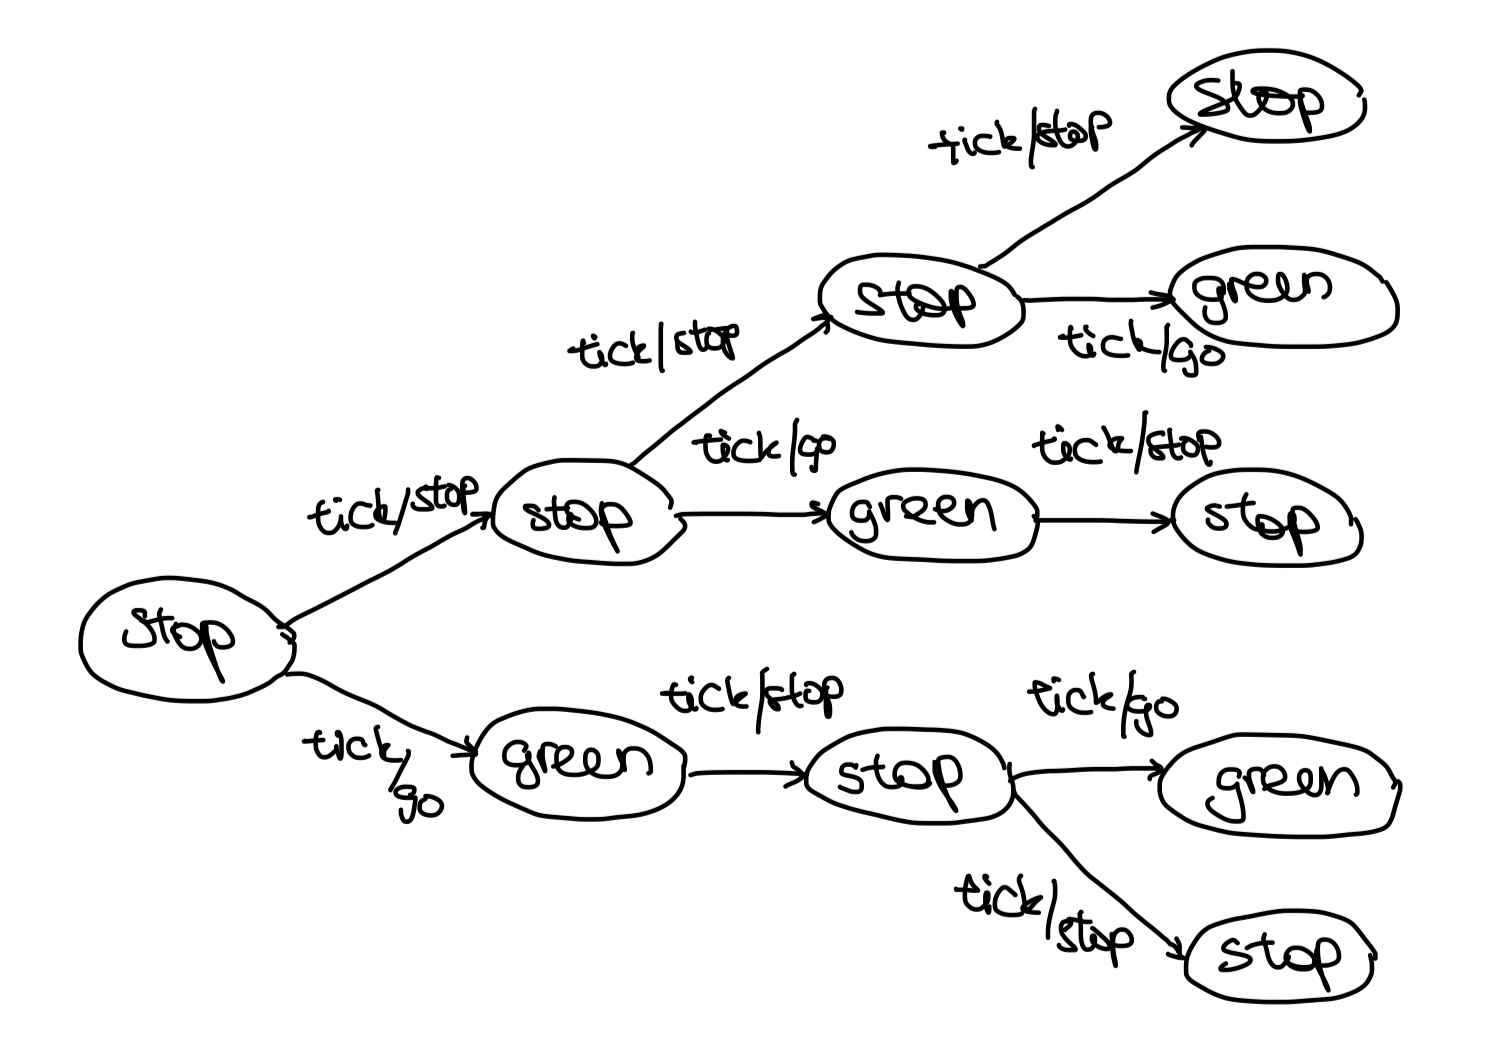
\includegraphics[width=9cm]{Ch3Ex5.jpeg}
    \caption{Trace prefix of length 4}
    \label{fig:Ch3Ex5}
    \end{figure}
\end{enumerate}

\section*{Chapter 5 - page }
\subsection*{Exercise 3 (10 marks)}
Figure \ref{fig:Ch5Ex3} below shows the single state machine $C$. The states (s2, s4), (s1, s5) and (s2, s5) highlighted in blue below are unreachable.
\begin{figure}[H]
    \centering
    \textbf{Input}: $a$: pure\\
    \textbf{Output}: $c$: pure\\
    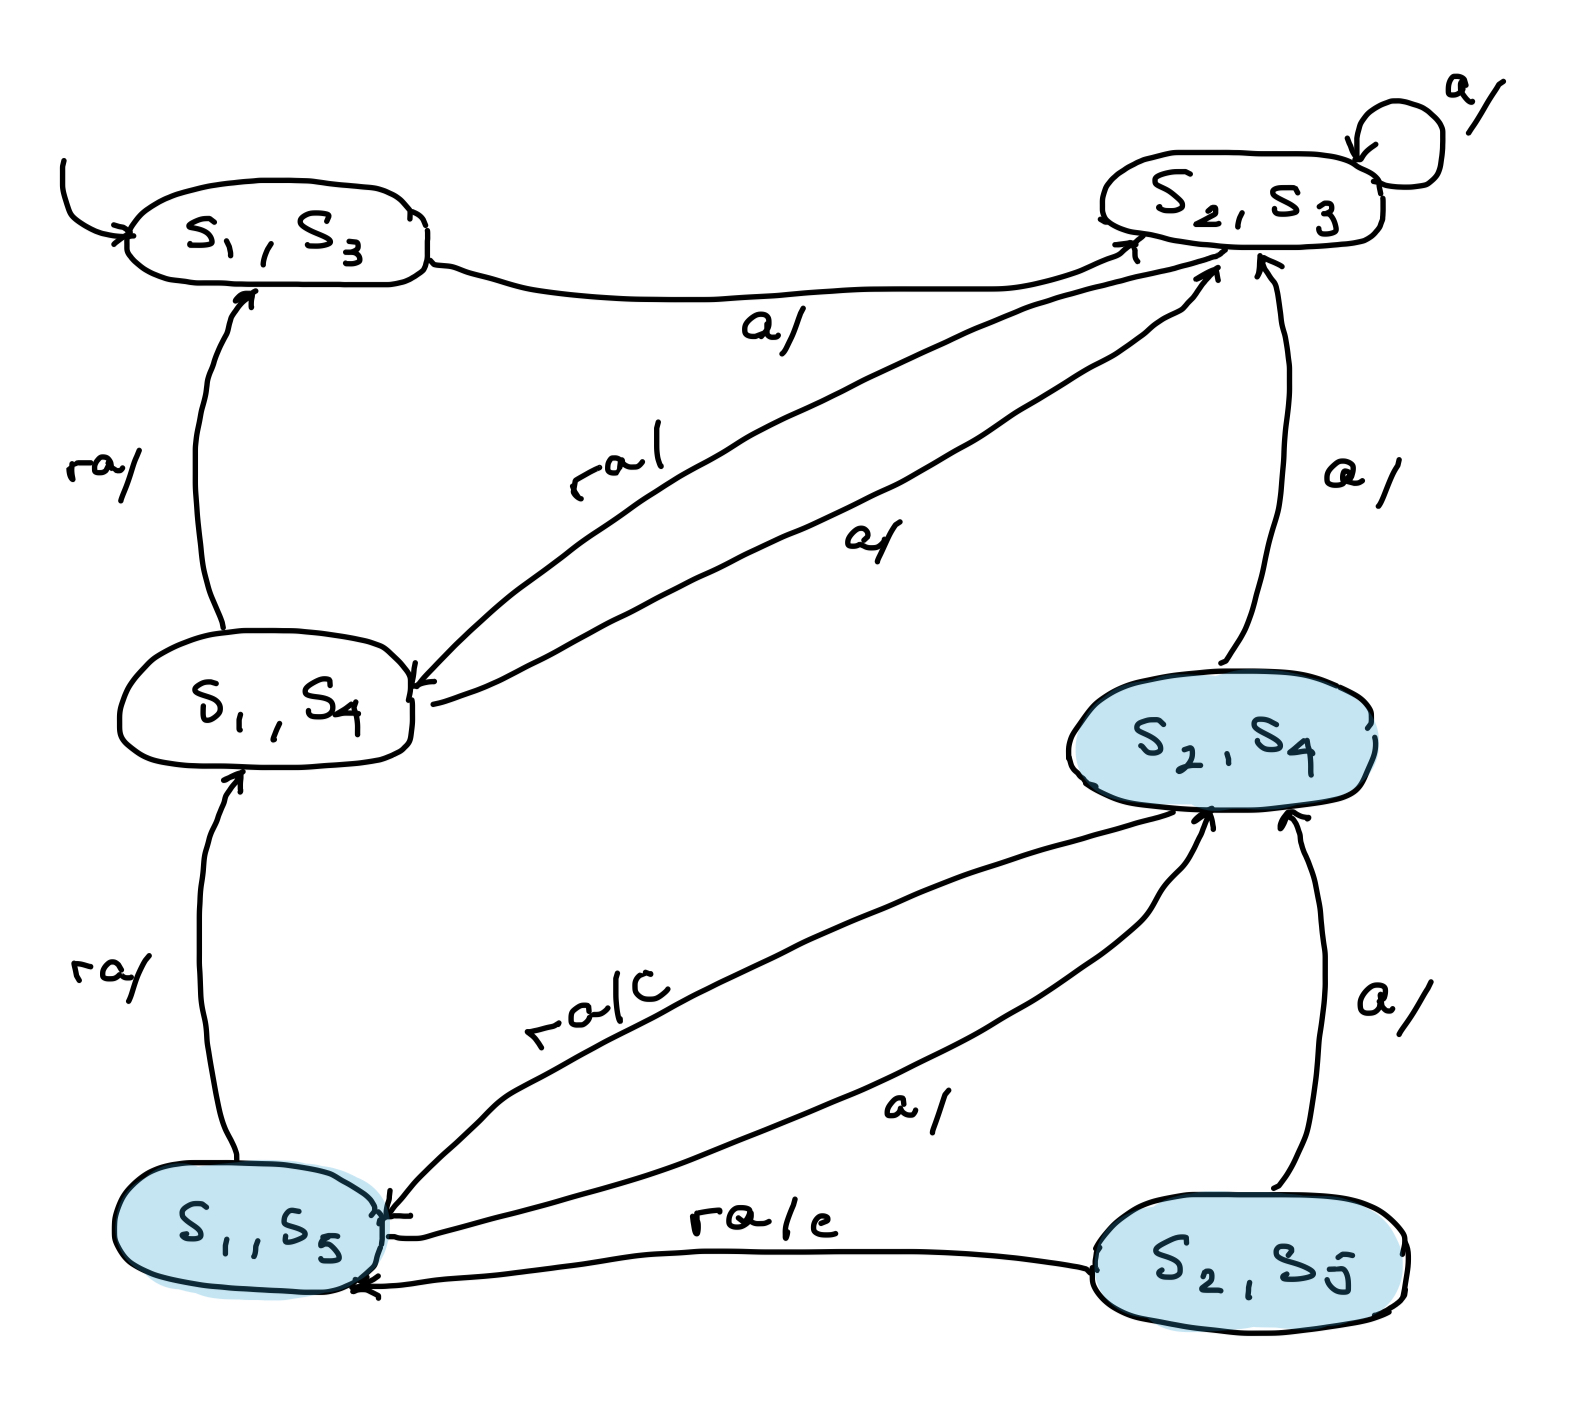
\includegraphics[width=6.5cm]{Ch5Ex3.jpeg}
    \caption{Combined state machine $C$}
    \label{fig:Ch5Ex3}
\end{figure}
\subsection*{Exercise 5 (7 marks)}
Figure \ref{fig:Ch5Ex5} below shows the flattened final state machine.  Unreachable states are left out from the drawing e.g. (D, E) or (D, F) because the reset transition will always go back to C. The machine A in this case is also simplified to C because the initial state for A defaults to C.
\begin{figure}[H]
    \centering
    \textbf{Input}: $a$: pure\\
    \textbf{Output}: $b$: pure\\
    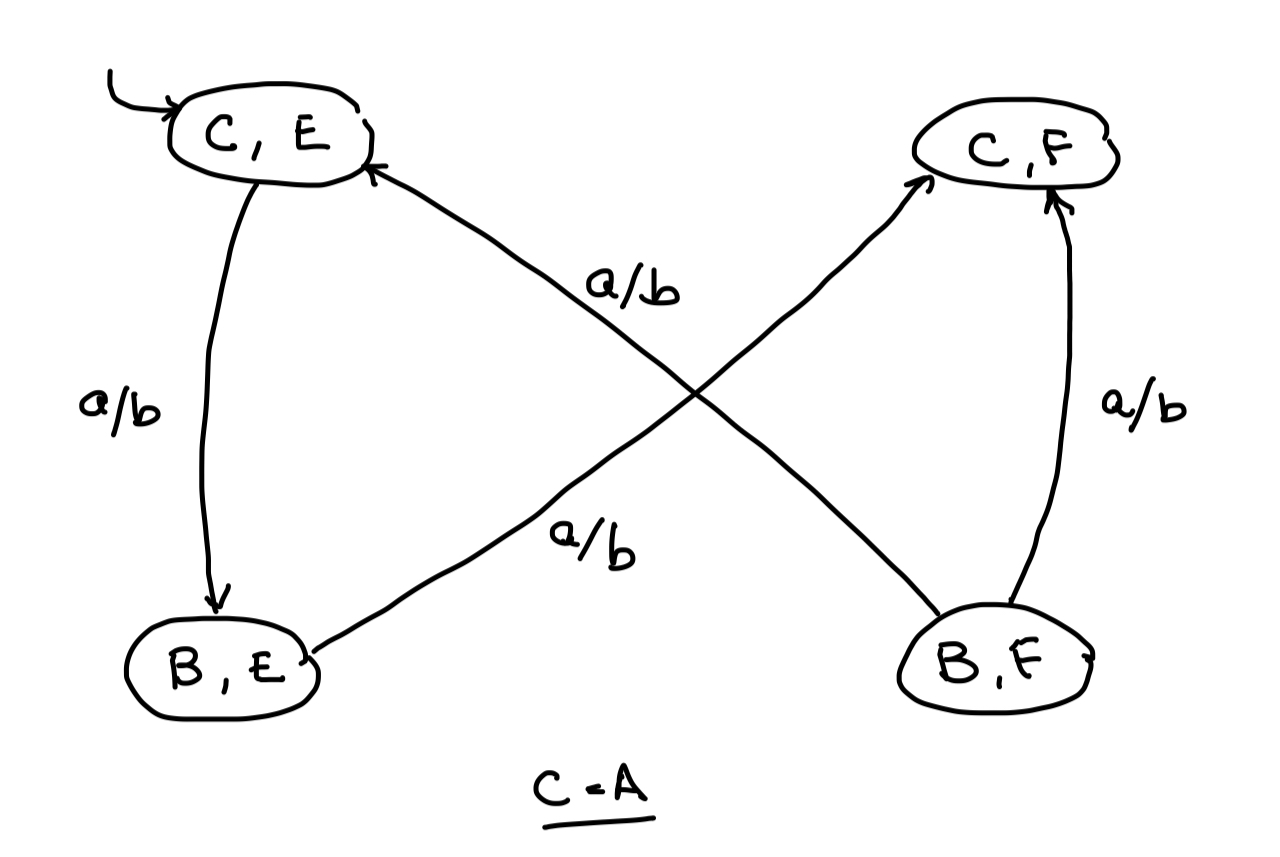
\includegraphics[width=6.2cm]{Ch5Ex5.jpeg}
    \caption{Flattened FSM}
    \label{fig:Ch5Ex5}
\end{figure}
The machine can be simplified easily into a single state machine taking in a present input $a$ to give output $b$. This is described in Figure \ref{fig:Ch5Ex5a}.
\begin{figure}[H]
    \centering
    \textbf{Input}: $a$: pure\\
    \textbf{Output}: $b$: pure\\
    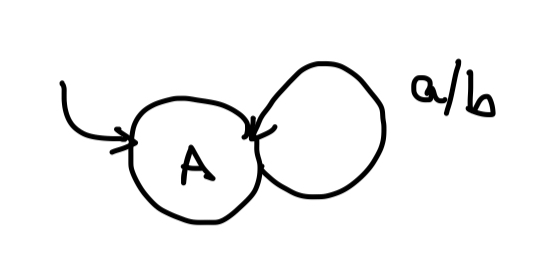
\includegraphics[width=2cm]{Ch5Ex5a.jpeg}
    \caption{Simplified state machine}
    \label{fig:Ch5Ex5a}
\end{figure}
\end{document}